
% Default to the notebook output style

    


% Inherit from the specified cell style.




    
\documentclass{article}

    
    
    \usepackage{graphicx} % Used to insert images
    \usepackage{adjustbox} % Used to constrain images to a maximum size 
    \usepackage{color} % Allow colors to be defined
    \usepackage{enumerate} % Needed for markdown enumerations to work
    \usepackage{geometry} % Used to adjust the document margins
    \usepackage{amsmath} % Equations
    \usepackage{amssymb} % Equations
    \usepackage{eurosym} % defines \euro
    \usepackage[mathletters]{ucs} % Extended unicode (utf-8) support
    \usepackage[utf8x]{inputenc} % Allow utf-8 characters in the tex document
    \usepackage{fancyvrb} % verbatim replacement that allows latex
    \usepackage{grffile} % extends the file name processing of package graphics 
                         % to support a larger range 
    % The hyperref package gives us a pdf with properly built
    % internal navigation ('pdf bookmarks' for the table of contents,
    % internal cross-reference links, web links for URLs, etc.)
    \usepackage{hyperref}
    \usepackage{longtable} % longtable support required by pandoc >1.10
    \usepackage{booktabs}  % table support for pandoc > 1.12.2
    \usepackage{indentfirst}
    \usepackage{amsmath}
    \usepackage{floatrow}
    
    
    \definecolor{orange}{cmyk}{0,0.4,0.8,0.2}
    \definecolor{darkorange}{rgb}{.71,0.21,0.01}
    \definecolor{darkgreen}{rgb}{.12,.54,.11}
    \definecolor{myteal}{rgb}{.26, .44, .56}
    \definecolor{gray}{gray}{0.45}
    \definecolor{lightgray}{gray}{.95}
    \definecolor{mediumgray}{gray}{.8}
    \definecolor{inputbackground}{rgb}{.95, .95, .85}
    \definecolor{outputbackground}{rgb}{.95, .95, .95}
    \definecolor{traceback}{rgb}{1, .95, .95}
    % ansi colors
    \definecolor{red}{rgb}{.6,0,0}
    \definecolor{green}{rgb}{0,.65,0}
    \definecolor{brown}{rgb}{0.6,0.6,0}
    \definecolor{blue}{rgb}{0,.145,.698}
    \definecolor{purple}{rgb}{.698,.145,.698}
    \definecolor{cyan}{rgb}{0,.698,.698}
    \definecolor{lightgray}{gray}{0.5}
    
    % bright ansi colors
    \definecolor{darkgray}{gray}{0.25}
    \definecolor{lightred}{rgb}{1.0,0.39,0.28}
    \definecolor{lightgreen}{rgb}{0.48,0.99,0.0}
    \definecolor{lightblue}{rgb}{0.53,0.81,0.92}
    \definecolor{lightpurple}{rgb}{0.87,0.63,0.87}
    \definecolor{lightcyan}{rgb}{0.5,1.0,0.83}
    
    % commands and environments needed by pandoc snippets
    % extracted from the output of `pandoc -s`
    \providecommand{\tightlist}{%
      \setlength{\itemsep}{0pt}\setlength{\parskip}{0pt}}
    \DefineVerbatimEnvironment{Highlighting}{Verbatim}{commandchars=\\\{\}}
    % Add ',fontsize=\small' for more characters per line
    \newenvironment{Shaded}{}{}
    \newcommand{\KeywordTok}[1]{\textcolor[rgb]{0.00,0.44,0.13}{\textbf{{#1}}}}
    \newcommand{\DataTypeTok}[1]{\textcolor[rgb]{0.56,0.13,0.00}{{#1}}}
    \newcommand{\DecValTok}[1]{\textcolor[rgb]{0.25,0.63,0.44}{{#1}}}
    \newcommand{\BaseNTok}[1]{\textcolor[rgb]{0.25,0.63,0.44}{{#1}}}
    \newcommand{\FloatTok}[1]{\textcolor[rgb]{0.25,0.63,0.44}{{#1}}}
    \newcommand{\CharTok}[1]{\textcolor[rgb]{0.25,0.44,0.63}{{#1}}}
    \newcommand{\StringTok}[1]{\textcolor[rgb]{0.25,0.44,0.63}{{#1}}}
    \newcommand{\CommentTok}[1]{\textcolor[rgb]{0.38,0.63,0.69}{\textit{{#1}}}}
    \newcommand{\OtherTok}[1]{\textcolor[rgb]{0.00,0.44,0.13}{{#1}}}
    \newcommand{\AlertTok}[1]{\textcolor[rgb]{1.00,0.00,0.00}{\textbf{{#1}}}}
    \newcommand{\FunctionTok}[1]{\textcolor[rgb]{0.02,0.16,0.49}{{#1}}}
    \newcommand{\RegionMarkerTok}[1]{{#1}}
    \newcommand{\ErrorTok}[1]{\textcolor[rgb]{1.00,0.00,0.00}{\textbf{{#1}}}}
    \newcommand{\NormalTok}[1]{{#1}}
    
    % Define a nice break command that doesn't care if a line doesn't already
    % exist.
    \def\br{\hspace*{\fill} \\* }
    % Math Jax compatability definitions
    \def\gt{>}
    \def\lt{<}
    % Document parameters
    \title{Homework 9}
    \author{Roly Vicar\'ia \\ STAT501 Fall 2015}    
    
    

    % Pygments definitions
    
\makeatletter
\def\PY@reset{\let\PY@it=\relax \let\PY@bf=\relax%
    \let\PY@ul=\relax \let\PY@tc=\relax%
    \let\PY@bc=\relax \let\PY@ff=\relax}
\def\PY@tok#1{\csname PY@tok@#1\endcsname}
\def\PY@toks#1+{\ifx\relax#1\empty\else%
    \PY@tok{#1}\expandafter\PY@toks\fi}
\def\PY@do#1{\PY@bc{\PY@tc{\PY@ul{%
    \PY@it{\PY@bf{\PY@ff{#1}}}}}}}
\def\PY#1#2{\PY@reset\PY@toks#1+\relax+\PY@do{#2}}

\expandafter\def\csname PY@tok@gd\endcsname{\def\PY@tc##1{\textcolor[rgb]{0.63,0.00,0.00}{##1}}}
\expandafter\def\csname PY@tok@gu\endcsname{\let\PY@bf=\textbf\def\PY@tc##1{\textcolor[rgb]{0.50,0.00,0.50}{##1}}}
\expandafter\def\csname PY@tok@gt\endcsname{\def\PY@tc##1{\textcolor[rgb]{0.00,0.27,0.87}{##1}}}
\expandafter\def\csname PY@tok@gs\endcsname{\let\PY@bf=\textbf}
\expandafter\def\csname PY@tok@gr\endcsname{\def\PY@tc##1{\textcolor[rgb]{1.00,0.00,0.00}{##1}}}
\expandafter\def\csname PY@tok@cm\endcsname{\let\PY@it=\textit\def\PY@tc##1{\textcolor[rgb]{0.25,0.50,0.50}{##1}}}
\expandafter\def\csname PY@tok@vg\endcsname{\def\PY@tc##1{\textcolor[rgb]{0.10,0.09,0.49}{##1}}}
\expandafter\def\csname PY@tok@m\endcsname{\def\PY@tc##1{\textcolor[rgb]{0.40,0.40,0.40}{##1}}}
\expandafter\def\csname PY@tok@mh\endcsname{\def\PY@tc##1{\textcolor[rgb]{0.40,0.40,0.40}{##1}}}
\expandafter\def\csname PY@tok@go\endcsname{\def\PY@tc##1{\textcolor[rgb]{0.53,0.53,0.53}{##1}}}
\expandafter\def\csname PY@tok@ge\endcsname{\let\PY@it=\textit}
\expandafter\def\csname PY@tok@vc\endcsname{\def\PY@tc##1{\textcolor[rgb]{0.10,0.09,0.49}{##1}}}
\expandafter\def\csname PY@tok@il\endcsname{\def\PY@tc##1{\textcolor[rgb]{0.40,0.40,0.40}{##1}}}
\expandafter\def\csname PY@tok@cs\endcsname{\let\PY@it=\textit\def\PY@tc##1{\textcolor[rgb]{0.25,0.50,0.50}{##1}}}
\expandafter\def\csname PY@tok@cp\endcsname{\def\PY@tc##1{\textcolor[rgb]{0.74,0.48,0.00}{##1}}}
\expandafter\def\csname PY@tok@gi\endcsname{\def\PY@tc##1{\textcolor[rgb]{0.00,0.63,0.00}{##1}}}
\expandafter\def\csname PY@tok@gh\endcsname{\let\PY@bf=\textbf\def\PY@tc##1{\textcolor[rgb]{0.00,0.00,0.50}{##1}}}
\expandafter\def\csname PY@tok@ni\endcsname{\let\PY@bf=\textbf\def\PY@tc##1{\textcolor[rgb]{0.60,0.60,0.60}{##1}}}
\expandafter\def\csname PY@tok@nl\endcsname{\def\PY@tc##1{\textcolor[rgb]{0.63,0.63,0.00}{##1}}}
\expandafter\def\csname PY@tok@nn\endcsname{\let\PY@bf=\textbf\def\PY@tc##1{\textcolor[rgb]{0.00,0.00,1.00}{##1}}}
\expandafter\def\csname PY@tok@no\endcsname{\def\PY@tc##1{\textcolor[rgb]{0.53,0.00,0.00}{##1}}}
\expandafter\def\csname PY@tok@na\endcsname{\def\PY@tc##1{\textcolor[rgb]{0.49,0.56,0.16}{##1}}}
\expandafter\def\csname PY@tok@nb\endcsname{\def\PY@tc##1{\textcolor[rgb]{0.00,0.50,0.00}{##1}}}
\expandafter\def\csname PY@tok@nc\endcsname{\let\PY@bf=\textbf\def\PY@tc##1{\textcolor[rgb]{0.00,0.00,1.00}{##1}}}
\expandafter\def\csname PY@tok@nd\endcsname{\def\PY@tc##1{\textcolor[rgb]{0.67,0.13,1.00}{##1}}}
\expandafter\def\csname PY@tok@ne\endcsname{\let\PY@bf=\textbf\def\PY@tc##1{\textcolor[rgb]{0.82,0.25,0.23}{##1}}}
\expandafter\def\csname PY@tok@nf\endcsname{\def\PY@tc##1{\textcolor[rgb]{0.00,0.00,1.00}{##1}}}
\expandafter\def\csname PY@tok@si\endcsname{\let\PY@bf=\textbf\def\PY@tc##1{\textcolor[rgb]{0.73,0.40,0.53}{##1}}}
\expandafter\def\csname PY@tok@s2\endcsname{\def\PY@tc##1{\textcolor[rgb]{0.73,0.13,0.13}{##1}}}
\expandafter\def\csname PY@tok@vi\endcsname{\def\PY@tc##1{\textcolor[rgb]{0.10,0.09,0.49}{##1}}}
\expandafter\def\csname PY@tok@nt\endcsname{\let\PY@bf=\textbf\def\PY@tc##1{\textcolor[rgb]{0.00,0.50,0.00}{##1}}}
\expandafter\def\csname PY@tok@nv\endcsname{\def\PY@tc##1{\textcolor[rgb]{0.10,0.09,0.49}{##1}}}
\expandafter\def\csname PY@tok@s1\endcsname{\def\PY@tc##1{\textcolor[rgb]{0.73,0.13,0.13}{##1}}}
\expandafter\def\csname PY@tok@kd\endcsname{\let\PY@bf=\textbf\def\PY@tc##1{\textcolor[rgb]{0.00,0.50,0.00}{##1}}}
\expandafter\def\csname PY@tok@sh\endcsname{\def\PY@tc##1{\textcolor[rgb]{0.73,0.13,0.13}{##1}}}
\expandafter\def\csname PY@tok@sc\endcsname{\def\PY@tc##1{\textcolor[rgb]{0.73,0.13,0.13}{##1}}}
\expandafter\def\csname PY@tok@sx\endcsname{\def\PY@tc##1{\textcolor[rgb]{0.00,0.50,0.00}{##1}}}
\expandafter\def\csname PY@tok@bp\endcsname{\def\PY@tc##1{\textcolor[rgb]{0.00,0.50,0.00}{##1}}}
\expandafter\def\csname PY@tok@c1\endcsname{\let\PY@it=\textit\def\PY@tc##1{\textcolor[rgb]{0.25,0.50,0.50}{##1}}}
\expandafter\def\csname PY@tok@kc\endcsname{\let\PY@bf=\textbf\def\PY@tc##1{\textcolor[rgb]{0.00,0.50,0.00}{##1}}}
\expandafter\def\csname PY@tok@c\endcsname{\let\PY@it=\textit\def\PY@tc##1{\textcolor[rgb]{0.25,0.50,0.50}{##1}}}
\expandafter\def\csname PY@tok@mf\endcsname{\def\PY@tc##1{\textcolor[rgb]{0.40,0.40,0.40}{##1}}}
\expandafter\def\csname PY@tok@err\endcsname{\def\PY@bc##1{\setlength{\fboxsep}{0pt}\fcolorbox[rgb]{1.00,0.00,0.00}{1,1,1}{\strut ##1}}}
\expandafter\def\csname PY@tok@mb\endcsname{\def\PY@tc##1{\textcolor[rgb]{0.40,0.40,0.40}{##1}}}
\expandafter\def\csname PY@tok@ss\endcsname{\def\PY@tc##1{\textcolor[rgb]{0.10,0.09,0.49}{##1}}}
\expandafter\def\csname PY@tok@sr\endcsname{\def\PY@tc##1{\textcolor[rgb]{0.73,0.40,0.53}{##1}}}
\expandafter\def\csname PY@tok@mo\endcsname{\def\PY@tc##1{\textcolor[rgb]{0.40,0.40,0.40}{##1}}}
\expandafter\def\csname PY@tok@kn\endcsname{\let\PY@bf=\textbf\def\PY@tc##1{\textcolor[rgb]{0.00,0.50,0.00}{##1}}}
\expandafter\def\csname PY@tok@mi\endcsname{\def\PY@tc##1{\textcolor[rgb]{0.40,0.40,0.40}{##1}}}
\expandafter\def\csname PY@tok@gp\endcsname{\let\PY@bf=\textbf\def\PY@tc##1{\textcolor[rgb]{0.00,0.00,0.50}{##1}}}
\expandafter\def\csname PY@tok@o\endcsname{\def\PY@tc##1{\textcolor[rgb]{0.40,0.40,0.40}{##1}}}
\expandafter\def\csname PY@tok@kr\endcsname{\let\PY@bf=\textbf\def\PY@tc##1{\textcolor[rgb]{0.00,0.50,0.00}{##1}}}
\expandafter\def\csname PY@tok@s\endcsname{\def\PY@tc##1{\textcolor[rgb]{0.73,0.13,0.13}{##1}}}
\expandafter\def\csname PY@tok@kp\endcsname{\def\PY@tc##1{\textcolor[rgb]{0.00,0.50,0.00}{##1}}}
\expandafter\def\csname PY@tok@w\endcsname{\def\PY@tc##1{\textcolor[rgb]{0.73,0.73,0.73}{##1}}}
\expandafter\def\csname PY@tok@kt\endcsname{\def\PY@tc##1{\textcolor[rgb]{0.69,0.00,0.25}{##1}}}
\expandafter\def\csname PY@tok@ow\endcsname{\let\PY@bf=\textbf\def\PY@tc##1{\textcolor[rgb]{0.67,0.13,1.00}{##1}}}
\expandafter\def\csname PY@tok@sb\endcsname{\def\PY@tc##1{\textcolor[rgb]{0.73,0.13,0.13}{##1}}}
\expandafter\def\csname PY@tok@k\endcsname{\let\PY@bf=\textbf\def\PY@tc##1{\textcolor[rgb]{0.00,0.50,0.00}{##1}}}
\expandafter\def\csname PY@tok@se\endcsname{\let\PY@bf=\textbf\def\PY@tc##1{\textcolor[rgb]{0.73,0.40,0.13}{##1}}}
\expandafter\def\csname PY@tok@sd\endcsname{\let\PY@it=\textit\def\PY@tc##1{\textcolor[rgb]{0.73,0.13,0.13}{##1}}}

\def\PYZbs{\char`\\}
\def\PYZus{\char`\_}
\def\PYZob{\char`\{}
\def\PYZcb{\char`\}}
\def\PYZca{\char`\^}
\def\PYZam{\char`\&}
\def\PYZlt{\char`\<}
\def\PYZgt{\char`\>}
\def\PYZsh{\char`\#}
\def\PYZpc{\char`\%}
\def\PYZdl{\char`\$}
\def\PYZhy{\char`\-}
\def\PYZsq{\char`\'}
\def\PYZdq{\char`\"}
\def\PYZti{\char`\~}
% for compatibility with earlier versions
\def\PYZat{@}
\def\PYZlb{[}
\def\PYZrb{]}
\makeatother


    % Exact colors from NB
    \definecolor{incolor}{rgb}{0.0, 0.0, 0.5}
    \definecolor{outcolor}{rgb}{0.545, 0.0, 0.0}



    
    % Prevent overflowing lines due to hard-to-break entities
    \sloppy 
    % Setup hyperref package
    \hypersetup{
      breaklinks=true,  % so long urls are correctly broken across lines
      colorlinks=true,
      urlcolor=blue,
      linkcolor=darkorange,
      citecolor=darkgreen,
      }
    % Slightly bigger margins than the latex defaults
    
    \geometry{verbose,tmargin=1in,bmargin=1in,lmargin=1in,rmargin=1in}
    
    

    \begin{document}
    
    
    \maketitle
    
    

    
    \subsubsection{Question 1}\label{question-1}

\begin{enumerate}
\def\labelenumi{\alph{enumi})}
\tightlist
\item
  The SLR models based on each single predictor, as well as the matrix
  plot below, indicate that the best linear predictors for Y are
  \(x_1\), \(x_3\), \(x_4\), and \(x_7\).
  
  \begin{figure}[h!]
 \centering
 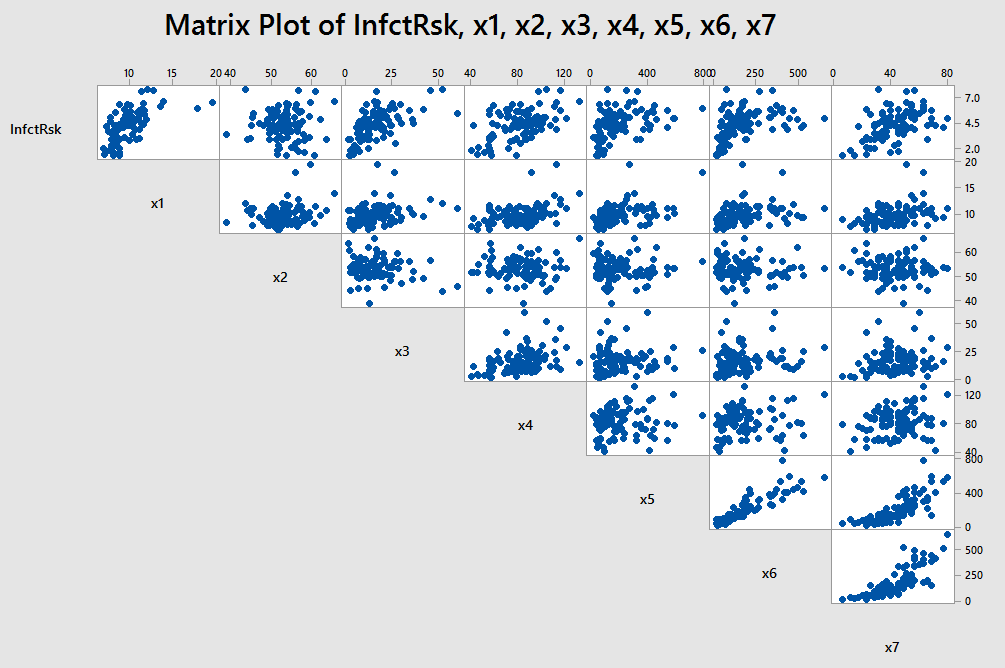
\includegraphics[scale=.5]{./images/matrix-plot_infectionRisk.png}
 % matrix-plot_infectionRisk.png: 1005x668 pixel, 96dpi, 26.59x17.67 cm, bb=0 0 754 501
\end{figure}
\end{enumerate}

\begin{enumerate}
\def\labelenumi{\alph{enumi})}
\setcounter{enumi}{1}
\tightlist
\item
  The ``best'' stepwise model selected the same 4 predictors from part
  (a).
  
  \begin{figure}[h!]
 \centering
 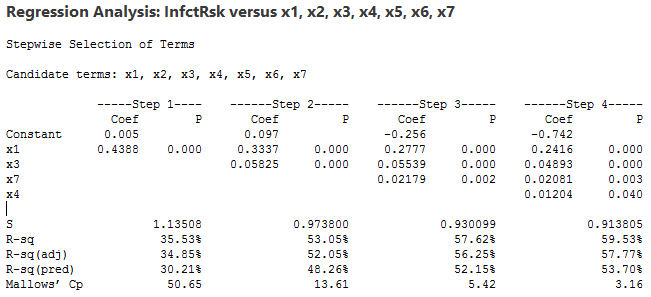
\includegraphics[scale=.6]{./images/stepwise_regression.png}
 % stepwise_regression.png: 651x297 pixel, 96dpi, 17.22x7.86 cm, bb=0 0 488 223
\end{figure}
\end{enumerate}

\begin{enumerate}
\def\labelenumi{\alph{enumi})}
\setcounter{enumi}{2}
\item
  Best subsets: \\
\begin{figure}[h!]
 \centering
 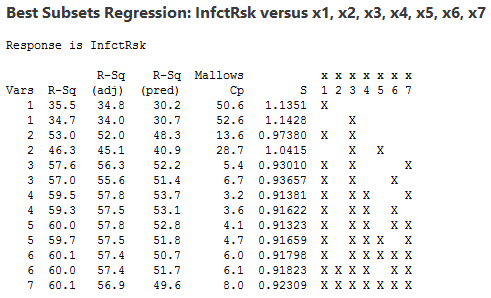
\includegraphics[scale=.6]{./images/best-subsets_regression.png}
 % best-subsets_regression.png: 491x298 pixel, 96dpi, 12.99x7.88 cm, bb=0 0 368 223
\end{figure}


  \begin{enumerate}
  \def\labelenumii{\roman{enumii}.}
  \tightlist
  \item
    Of the two 4-predictor models listed, there was a very small
    difference in terms of their adjusted \(R^2\) and \(C_p\) criterion.
    The better of the two was the model consisting of \(x_1\), \(x_3\),
    \(x_4\), and \(x_7\).
  \item
    Of the two 5-predictor models listed, there was again a very small
    difference in terms of their adjusted \(R^2\) and \(C_p\) criterion.
    The better of the two was the model consisting of \(x_1\), \(x_3\),
    \(x_4\), \(x_6\), and \(x_7\).
  \end{enumerate}
\item
  The test here is whether \(\beta_6 = 0\).
  \(H_0: \beta_6 = 0, H_a: \beta_6 \ne 0\)

\begin{align*}
df_R &= n - p = 97 - 5 = 92 \\
MSE_R &= S_R^2 = 0.91381^2 \approx 0.83505 \\
SSE_R &= MSE_R * (n - p) = 0.83505 * (97 - 5) \approx 76.8245 \\
\\
df_F &= n - p = 97 - 6 = 91 \\ 
MSE_F &= S_F^2 = 0.91323^2 \approx 0.833989 \\
SSE_F &= MSE_F * (n - p) = 0.833989 * (97 - 6) \approx 75.8930 \\
\\
F^* &= \frac{SSE_R - SSE_F}{df_R - df_F} \div \frac{SSE_F}{df_F} \\
    &= \frac{76.8245 - 75.8930}{92 - 91} \div \frac{75.8930}{91} \\
    &= 1.11692 \\
    \\
P(F > 1.11692) &= 0.293384
\end{align*}
%p-value: 1 - 0.706616 = 0.293384

Therefore, we fail to reject the null hypothesis and conclude that
\(x_6\) is not a significant predictor of Y and can be removed from the
model that already contains \(x_1\), \(x_3\), \(x_4\), and \(x_7\).
\end{enumerate}

\begin{enumerate}
\def\labelenumi{\alph{enumi})}
\setcounter{enumi}{4}
\item
  \begin{enumerate}
  \def\labelenumii{\roman{enumii}.}
  \tightlist
  \item
    Based on the stepwise and best subsets procedures, it looks like
    either \(x_1\) or \(x_3\) would be the most significant predictor.
    Out of the 13 models listed in the best subsets output, \(x_3\)
    appears in 12 of them, whereas \(x_1\) appears in 11 of them.
    \(x_1\) was the strongest individual predictor, so if I had to
    choose one, I would say \(x_1\) is the most significant.
  \item
    The ``best'' model that includes predictor \(x_6\) is the model that
    consists of \(x_1\), \(x_3\), \(x_4\), \(x_6\), and \(x_7\). It has
    the highest adjusted \(R^2\) value and lowest S value. It also has a
    good \(C_p\) value less than \(p\).
  \end{enumerate}
  \newpage
\item
  Some useful information found in the Stepwise procedure that is not
  found in the Best Subsets procedure, is the value of the coefficients
  and the \emph{p}-value of each parameter at each step of the process.
  Therefore, you can see the effect of the addition (or removal) of
  another parameter on the \emph{p}-value of a given parameter.

  Some useful information found in the Best Subsets procedure that is not
available in the Stepwise procedure is that it gives a ``larger
picture'' of possible models that are worth evaluating. The Stepwise
procedure seems a little more narrow in its output, where it basically
gives a single ``recommendation''. The minitab output for Stepwise
basically shows 4 candidate models, whereas the Best Subsets output
shows 13.
\end{enumerate}

\begin{enumerate}
\def\labelenumi{\alph{enumi})}
\setcounter{enumi}{6}
\item
  The ``best'' model with interaction effects chosen by the Stepwise
  procedure was the model that consists of \(x_1\), \(x_3\), \(x_4\),
  and \(x_7\) plus the addition of the interaction term \(x_3*x_7\).
\item
  \(C_p = p + \frac{(MSE_p - MSE_{all})(n - p)}{MSE_{all}} = 6 + \frac{(.7380 - .7514)(97 - 6)}{.7514} = 4.37716\)
  
  Based on this value of \(C_p\), it is unbiased.
\end{enumerate}

    \subsubsection{Question 2}\label{question-2}

\begin{enumerate}
\def\labelenumi{\alph{enumi})}
\tightlist
\item
  Model A:
  \(R_{adj}^2 = 1 - \left(\frac{n-1}{n-p}\right)\frac{SSE_p}{SSTO} = 1 - \left(\frac{99}{95}\right)\frac{1300}{5200} = 0.73947\) \\
\\
  Model B:
\(R_{adj}^2 = 1 - \left(\frac{n-1}{n-p}\right)\frac{SSE_p}{SSTO} = 1 - \left(\frac{99}{94}\right)\frac{1210}{5200} = 0.75493\)
\end{enumerate}

\begin{enumerate}
\def\labelenumi{\alph{enumi})}
\setcounter{enumi}{1}
\tightlist
\item
  Model A: \\
  \(AIC_p = n\ln(SSE_p) - n\ln(n) + 2p = 100\ln(1300) - 100\ln(100) + 2(5) = 266.4949\) \\
  \(BIC_p = n\ln(SSE_p) - n\ln(n) + p\ln(n) = 100\ln(1300) - 100\ln(100) + 5\ln(100) = 279.5208\) \\
  \\
  Model B: \\
  \(AIC_p = n\ln(SSE_p) - n\ln(n) + 2p = 100\ln(1210) - 100\ln(100) + 2(6) = 261.3206\) \\
  \(BIC_p = n\ln(SSE_p) - n\ln(n) + p\ln(n) = 100\ln(1210) - 100\ln(100) + 6\ln(100) = 276.9516\)
  
\end{enumerate}

\begin{enumerate}
\def\labelenumi{\alph{enumi})}
\setcounter{enumi}{2}
\tightlist
\item
  \(MSE_{all} = \frac{SSE_{all}}{n - p} = \frac{1150}{100-11} = 12.9213\)\\
  \\
  Model A:
  \(C_p = \frac{SSE_p}{MSE_{all}} - (n - 2p) = \frac{1300}{12.9213} - (100 - 2*5) = 10.6091\)\\
\\
  Model B:
  \(C_p = \frac{SSE_p}{MSE_{all}} - (n - 2p) = \frac{1210}{12.9213} - (100 - 2*6) = 5.6438\)\\
\\
The \(C_p\) value of Model A is not desirable since it's double the
value of \emph{p}, it indicates bias. The \(C_p\) value of Model B is
near to the value of \emph{p} which is desirable.
\end{enumerate}

\begin{enumerate}
\def\labelenumi{\alph{enumi})}
\setcounter{enumi}{3}
\tightlist
\item
  Model B looks to be the preferable model across all criteria. It has a
  slightly higher adjusted \(R^2\) value and slightly lower information
  criterion values. However, I think the \(C_p\) is the deciding factor
  in the comparison. The \(C_p\) value for Model A is almost double the
  number of parameters while it's near the value of \emph{p} for Model
  B.
\end{enumerate}

\newpage
    \subsubsection{Question 3}\label{question-3}

\begin{enumerate}
\def\labelenumi{\alph{enumi})}
\item
\end{enumerate}

\begin{longtable}[c]{@{}lllllllll@{}}
\toprule
Vars & R-sq & R-sq (adj) & Mallows' \(C_p\) & S & 1 & 2 & 3 &
4\tabularnewline
\midrule
\endhead
1 & 68.411 & 67.753 & 2.082 & 2.413 & & & X &\tabularnewline
1 & 64.184 & 63.438 & 8.516 & 2.569 & & X & &\tabularnewline
2 & 70.332 & 69.070 & 1.157 & 2.363 & & X & X &\tabularnewline
2 & 69.112 & 67.797 & 3.015 & 2.411 & & & X & X\tabularnewline
3 & 70.434 & 68.506 & 3.003 & 2.385 & X & X & X &\tabularnewline
3 & 70.366 & 68.434 & 3.106 & 2.387 & & X & X & X\tabularnewline
4 & 70.434 & 67.806 & 5.003 & 2.411 & X & X & X & X\tabularnewline
\bottomrule
\end{longtable}

\begin{enumerate}
\def\labelenumi{\alph{enumi})}
\setcounter{enumi}{1}
\tightlist
\item
  From the table in part (a), we can see that the models are all very
  close in terms of their R-sq values and being unbiased models (with
  the exception of row 2). Starting from the model consisting of
  \(x_3\), there was marginal improvement by adding \(x_2\) to it.
  Without having any additional context about the purpose of the model,
  this seems like one of those situations where it would be best to opt
  for the simpler model since it doesn't look like there is much benefit
  from choosing a more complicated model. So from that point of view, I
  would conclude that the model consisting of the single predictor
  \(x_3\), would be the ``best'' choice of those listed.
\end{enumerate}


    % Add a bibliography block to the postdoc
    
    
    
    \end{document}
